\documentclass{article}
\newcommand{\BEAS}{\begin{eqnarray*}}
\newcommand{\EEAS}{\end{eqnarray*}}
\newcommand{\BEQ}{\begin{equation}}
\newcommand{\EEQ}{\end{equation}}
\newcommand{\BIT}{\begin{itemize}}
\newcommand{\EIT}{\end{itemize}}

\newcommand{\eg}{{\it e.g.\ }}
\newcommand{\ie}{{\it i.e.\ }}

\newcommand{\ones}{\mathbf 1}
\newcommand{\zeros}{\mathbf 0}
\newcommand{\reals}{{\mbox{\bf R}}}
\newcommand{\integers}{{\mbox{\bf Z}}}
\newcommand{\symm}{{\mbox{\bf S}}}  % symmetric matrices

\newcommand{\nullspace}{{\mathcal N}}
\newcommand{\range}{{\mathcal R}}
\newcommand{\Rank}{\mathop{\bf Rank}}
\newcommand{\Tr}{\mathop{\bf Tr}}

\newcommand{\sign}[1]{\mathop{\textrm{sgn}}(#1)}
\newcommand{\lambdamax}{{\lambda_{\rm max}}}
\newcommand{\lambdamin}{\lambda_{\rm min}}

\newcommand{\EE}{\mathop{\textrm{E}}}
\newcommand{\Cov}{\mathop{\textrm{Cov}}}
\newcommand{\Prob}{\mathop{\bf Prob}}
\newcommand{\Co}{{\mathop {\bf Co}}} % convex hull
\newcommand{\dist}{\mathop{\bf dist{}}}
\newcommand{\argmin}{\mathop{\rm argmin}}
\newcommand{\argmax}{\mathop{\rm argmax}}
\newcommand{\epi}{\mathop{\bf epi}} % epigraph
\newcommand{\Vol}{\mathop{\bf vol}}
\newcommand{\dom}{\mathop{\bf dom}} % domain
\newcommand{\intr}{\mathop{\bf int}}


\newcommand{\nrm}[1]{\left\lVert#1\right\rVert}
\newcommand{\nrmo}[1]{\left\lVert#1\right\rVert_1}
\newcommand{\nrmt}[1]{\left\lVert#1\right\rVert_2}
\newcommand{\nrmnn}[1]{\left\lVert#1\right\rVert_{*}}
\newcommand{\nrmf}[1]{\left\lVert#1\right\rVert_F}

\newcommand{\myexp}[1]{\mathop{\rm exp}\left\{#1\right\}}
\newcommand{\mylog}[1]{\mathop{\rm log}\left\{#1\right\}}
\newcommand{\questions}{\begin{frame}Questions?\end{frame}}
\newcommand{\LL}{\textrm{LL}}
\newcommand{\KL}{\textrm{KL}}
\newcommand{\HH}{\textrm{H}}
\newcommand{\GG}{\textrm{G}}

\newcommand{\Bound}{\textrm{B}}
\newcommand{\bb}{\mathbf{b}}
\newcommand{\aaa}{\mathbf{a}}
\newcommand{\BB}{\mathbf{B}}
\newcommand{\AAA}{\mathbf{A}}
\newcommand{\CC}{\mathbf{C}}
\newcommand{\cc}{\mathbf{c}}
\newcommand{\mm}{\mathbf{m}}
\newcommand{\MM}{\mathbf{M}}
\newcommand{\nn}{\mathrm{\bf neighbors}}
\newcommand{\pa}[1]{{\textrm{\bf pa}}\left(#1\right)}
\newcommand{\pre}[2]{\mathop{\textrm{\bf pnp}}_{#1}\left(#2\right)}
\newcommand{\logsum}{\textrm{logsum}}

\newcommand{\tth}{{\textrm{th}}}
\newcommand{\xx}{\mathbf{x}}
\newcommand{\mmu}{\mathbf{\mu}}
\newcommand{\yy}{\mathbf{y}}
\newcommand{\zz}{\mathbf{z}}
\newcommand{\dd}{\mathbf{d}}
\newcommand{\new}{\textrm{new}}
\newcommand{\old}{\textrm{old}}
\newcommand{\fpr}{\textrm{FPR}}
\newcommand{\tpr}{\textrm{TPR}}
\newcommand{\auc}{\textrm{AUC}}
\newcommand{\yyi}{\yy_i}
\newcommand{\xxi}{\xx_i}
\newcommand{\vvec}[2]{\left[ \begin{array}{c} \mathbf{#1}\\ \mathbf{#2} \end{array}\right]}
\newcommand{\mmat}[4]{\left[ \begin{array}{cc} \mathbf{#1}&\mathbf{#2}\\ \mathbf{#3}&\mathbf{#4} \end{array}\right]}
\newcommand{\xyvec}{\left[ \begin{array}{c} \xx\\\yy \end{array} \right]}
\newcommand{\xyvecc}{\left[ \begin{array}{c} x^1\\y^1 \end{array} \right]}
\newcommand{\eye}{   \left[ \begin{array}{cc} 1 & 0 \\ 0 & 1 \end{array}\right]}
\newcommand{\bket}[2]{\left\langle#1,#2\right\rangle}
\newcommand{\bbket}[2]{\left\llangle#1,#2\right\rrangle}
\newcommand{\redq}{\textcolor{red}{q}}
\newcommand{\blup}{\textcolor{blue}{p}}
\newcommand{\BIEA}{\begin{IEEEeqnarray*}}
\newcommand{\EIEA}{\end{IEEEeqnarray*}}
\newcommand{\BIEAN}{\begin{IEEEeqnarray}}
\newcommand{\EIEAN}{\end{IEEEeqnarray}}
\newcommand{\pmin}{\mathop{\textrm{minimize}}}
\newcommand{\psubjto}{\textrm{subject to}}
\newcommand{\WW}{\mathbf{W}}
\newcommand{\ww}{\mathbf{w}}
\newcommand{\YY}{\mathbf{Y}}
\newcommand{\XX}{\mathbf{X}}
\newcommand{\UU}{\mathbf{U}}
\newcommand{\uu}{\mathbf{u}}
\newcommand{\VV}{\mathbf{V}}
\newcommand{\vv}{\mathbf{v}}
\newcommand{\PP}{\mathbf{P}}
\newcommand{\pp}{\mathbf{p}}
\newcommand{\rr}{\mathbf{r}}
\newcommand{\RR}{\mathbf{R}}
\newcommand{\ee}{\mathbf{e}}
\newcommand{\BA}{\mathbf{A}}

\newcommand{\aalpha}{{\boldsymbol\alpha}}
\newcommand{\llambda}{{\boldsymbol\lambda}}
\newcommand{\ddelta}{{\boldsymbol\delta}}
\newcommand{\otherwise}{\textrm{otherwise}}
\newcommand{\answer}{\fbox{\tt answer} }
\newcommand{\abs}[1]{\left| #1 \right|}

\newcounter{problemCtr}
\newcommand{\newproblem}[1]{\hrule\paragraph{Problem \theproblemCtr (#1)}\stepcounter{problemCtr}}


\newcounter{HW}

\usepackage{amsthm}
\usepackage{graphicx}
\usepackage{natbib}
\usepackage{algorithm}
\usepackage{algorithmic}
\usepackage{amsmath}
\usepackage{hyperref}


\newtheorem{remark}{Remark}
\newtheorem{lemma}{Lemma}
\newtheorem{definition}{Definition}
\newtheorem{proposition}{Proposition}
\newtheorem{assumption}{Assumption}
\newtheorem{corollary}{Corollary}
\newtheorem{theorem}{Theorem}


\begin{document}
\author{Chun-Wei Liu}
\setcounter{HW}{3}
\title{COMP  790-124, HW\theHW}
\maketitle

{ Deadline: 12/6/2014 11:59PM EST}

{ Submit \texttt{hw\theHW.pdf} by e-mail,  \url{mailto:vjojic+comp790+hw\theHW@cs.unc.edu}}.

\hrule

\section{Getting the data}

The homework archive has a separate subdirectory with Matlab scripts you need to get started, called \texttt{work}.
From \url{http://yann.lecun.com/exdb/mnist/} download:
\begin{itemize}
\item \texttt{train-images-idx3-ubyte.gz}
\item \texttt{train-labels-idx1-ubyte.gz}
\end{itemize}
decompress these files and add them to your work directory.
In Matlab change to the work directory and do following
\begin{verbatim}
mnistData   = loadMNISTImages('train-images.idx3-ubyte');
mnistLabels = loadMNISTLabels('train-labels.idx1-ubyte');
imagesc(reshape(mnistData(:,1),[28 28]))
colormap(gray)
mnistLabels(1)
\end{verbatim}
You should see an image of handwritten digit 5 and this should match printed value for \texttt{mnistLabels(1)}.


\section{Neural network architecture}

We will develop a method for digit recognition. The data will consist of examples of handwritten
digits of size $28 \times 28$ gray pixels, each such image labeled with digit that it corresponds to.
We will use a neural network consisting of four layers.

\pgfdeclarelayer{background}
\pgfdeclarelayer{foreground}
\pgfsetlayers{background,main,foreground}
\begin{figure}
\begin{center}
\begin{tikzpicture}[->,shorten >=0pt,auto,node distance=2cm,semithick]

\tikzstyle{var}=[minimum size=.7cm,circle,fill=white,draw=black,text=black]
\tikzstyle{ovar}=[minimum size=.7cm,circle,fill=gray,draw=black,text=black]
\tikzstyle{spacing}=[minimum size=.7cm,circle,fill=none,draw=none,text=black]

\node[ovar] (d41) {$h_{4,1}$};
\node[ovar] (d42) [right of=d41] {$h_{4,2}$};
\node[spacing] (d43) [right of=d42] {$\dots$};
\node[ovar] (d44) [right of=d43] {$h_{4,10}$};

\node[var] (d31) [below of=d41] {$h_{3,1}$};
\node[var] (d32) [below of=d42] {$h_{3,2}$};
\node[spacing] (d33) [right of=d32] {$\dots$};
\node[var] (d34) [right of=d33] {$h_{3,n_3}$};


\node[var] (d21) [below of=d31] {$h_{2,1}$};
\node[var] (d22) [below of=d32] {$h_{2,2}$};
\node[spacing] (d23) [right of=d22] {$\dots$};
\node[var] (d24) [right of=d23] {$h_{2,n_2}$};


\node[ovar] (d11) [below of=d21] {$h_{1,1}$};
\node[ovar] (d12) [below of=d22] {$h_{1,2}$};
\node[spacing] (d13) [right of=d12] {$\dots$};
\node[ovar] (d14) [right of=d13] {$h_{1,784}$};

\begin{pgfonlayer}{background}


\path (d11) edge (d21);\path (d12) edge (d21);\path (d14) edge (d21);
\path (d11) edge (d22);\path (d12) edge (d22);\path (d14) edge (d22);
\path (d11) edge (d24);\path (d12) edge (d24);\path (d14) edge  [right] node {$w^2_{n_2,784}$} (d24);

\path (d21) edge (d31);\path (d22) edge (d31);\path (d24) edge (d31);
\path (d21) edge (d32);\path (d22) edge (d32);\path (d24) edge (d32);
\path (d21) edge (d34);\path (d22) edge (d34);\path (d24) edge (d34);

\path (d31) edge (d41);\path (d32) edge (d41);\path (d34) edge (d41);
\path (d31) edge (d42);\path (d32) edge (d42);\path (d34) edge (d42);
\path (d31) edge (d44);\path (d32) edge (d44);\path (d34) edge (d44);

\end{pgfonlayer}
\end{tikzpicture}
\end{center}
\caption{Network is composed of 4 layers. Bottom layer corresponds to a handwritten digit image, one node per pixel of the 28 by 28 image.
Top layer is composed of 10 indicator variables, one for each possible digit. Two neighboring layers are densely connected. We label a single
edge to illustrate notation for weights. Additional details are provided in text.
\label{fig:nn}}
\end{figure}
The top layer is composed of indicator variables, one for every digit. Only one of those
variables is 1, the rest will be zero. So, if $h_{1,i} = 1$ then the digit is $i-1$.

The bottom layer is composed of pixel intensity variables. Since images are of size 28 by 28, the
total number of variables in that layer is 784.

We use $n_l$ to denote number of nodes in layer $l$ where they are not know ahead of time.
In Fig.~\ref{fig:nn} one of the edges is labeled by its weight,$w^2_{n_2,784}$. We use $w^l_{i,j}$ to denote a weight of
 input from node $j$ in layer $l-1$ to node $i$ in layer l.

Each layer is densely connected to neighboring layers.


\section{Notation\label{sec:notation}}
 We will adopt notation whereby layer index is denoted in the superscript and subscript indices refer to nodes
\begin{itemize}
\item $w^l_{i,j}$ weight of connection between node $j$ in layer $l-1$ and node $i$ in layer $l$
\item $b^l_i$ is bias of node $i$ in layer $l$
\item $f^L$ is softmax, $f^{L-1},... f^2$ are unit activation functions
\item input to node $i$ in layer $l$
\begin{equation}\label{eq:a}
a^l_{i} = \sum_j w^l_{i,j}o^{l-1}_{j} + b^l_i
\end{equation}
\item output from node $i$ in layer $l$
\begin{equation} \label{eq:o}
o^l_{i} = f^l(a^l_{i})
\end{equation}
\end{itemize}
Hence $o^1_{j}$ is intensity of $j^\tth$ pixel in the image of a handwritten digit, and $o^L_{j}$ is an indicator of whether the handwritten digit is $j-1$.
Note that the first layer does not have corresponding $\ww$ or $b$ values because it is not modeled -- we assume that image pixel intensities are known.
We will use $n_l$ to denote number of nodes in layer $l$.

We will reserve index $t$ to indicate sample index. Note that activations and outputs may differ for different samples. Where
 relevant we will use $a^{l,t}_{i},o^{l,t}_i$ to denote sample specific analogs of the input and output variables defined above.
 Finally, $x^T$ will denote transposed vector, and $f'(x)$ will denote first derivative of a univariate function.

 \newproblem{1pt} Using $n_l$ and definitions of different variables in the notation Section~\ref{sec:notation} give their counts
 \begin{itemize}
  \item $\bb^l$ is a vector of size $n_l \times 1$
 \item $\WW^l$ is a matrix of size $n_l \times n_{l-1}$ 
 \item $\aaa^l$ is a vector of size $n_l \times 1$
\item $\oo^l$ is a vector of size $n_l \times 1$ 
\end{itemize}
\section{Softmax activation function}
Softmax activation function is given by
\begin{equation}
f_k(\aaa) = \frac{\myexp{a_k}}{\sum_{c=1}^C \myexp{a_c}}
\label{eq:softmaxact}
\end{equation}
where $k \in \{1,...,C\}$.

Using \eqref{eq:a} we can write
\begin{equation}
o^l_k = \frac{\myexp{(\ww^L_k)^T\oo^{l-1}}}{\sum_{c=1}^C\myexp{(\ww^L_c)^T\oo^{l-1}}} \label{eq:softmaxo}
\end{equation}
Note the sum of exponential functions, this should always signal use of log-sum.


\section{Rectified linear activation function}
A rectified linear unit activation function has following form:
\[
f(a) = \max(0, a)
\]
\newproblem{1pt}
Plot this function on a interval [-1,1] and replace \texttt{emptiness.pdf} with appropriate pdf below.
\begin{figure}[H]
\begin{center}
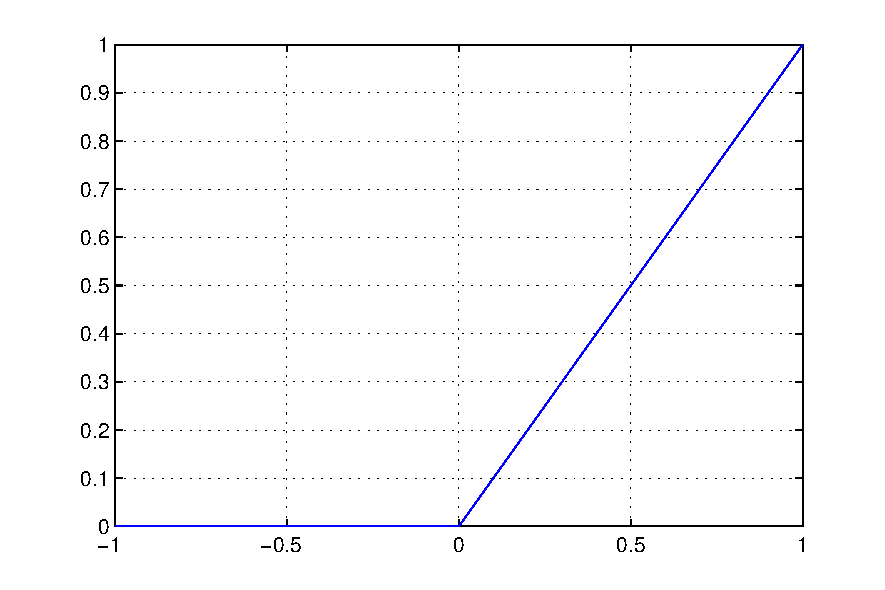
\includegraphics[scale=0.5]{relu.pdf}

\caption{This is a rectified linear activation function from -1 to 1.
\label{fig:relu}}

\end{center}
\end{figure}
\hrule

\section{Forward Propagation}
In our network forward propagation starts from the layer with pixel intensities and propagates activations
through the rectified linear units (ReLUs), and finally through softmax.
Specifically, activation functions for each layer are
\BEAS
f^2(a) = f^3(a) &=& \max(0,a) \\
f^4_k(\aaa) &=& \frac{\myexp{a_k}}{\sum_{c=1}^C \myexp{a_c}}
\EEAS
ReLU units in a single layer produce outputs independently of each other.
However, softmax units produce outputs jointly and depend on all the inputs into their layer, whole vector $\aaa$. This is due to the denominator depending on all $a_c$s.
It stands to reason, since the softmax units will sum up to 1, and hence are not be independent.

\newproblem{1pt}
Implement a function that takes performs forward propagation in the above network.
It should return outputs of each layer of neural net. You only need to implement propagation for ReLU units (layers 2 through L-1).


\begin{verbatim}
function os = forwardProp(data,layerwiseParams,architecture)
L = length(architecture);

os = cell(L,1);
os{1} = data;
N = size(data,2);
% relu propagation
for l=2:L-1
    W = layerwiseParams(l).w;
    b = layerwiseParams(l).b;
    a = W*os{l-1} + repmat(b,[1 N]);
    os{l} = max(0,a) % implement activation function of for
                     % rectified linear unit
end

% softmax
softmaxW = layerwiseParams(L).w;
C = architecture(L).size; % number of classes
o = softmaxW * os{L-1};
o = o - repmat(max(o,[],1),[C 1]);
o = exp(o);
o = o./repmat(sum(o),[C 1]);
os{L} = o;
\end{verbatim}

In the case of digits, data is a matrix of size $784 \times N$.
Note that propagation is performed for all samples simultaneously using matrix multiplication -- there is no {\texttt{for}} loop over samples.

Look at script \texttt{wrk.m} for examples of input provided to this code.

\hrule

\section{Loss function}
Next we will formulate a loss function that will tell us how good is our neural
network in predicting the digits.

\newproblem{1pt} Loss function for softmax model for a single sample  is given by
\BEAS
E_t(\WW) &=& \sum_{c=1}^C [y^t = c]\log o^{L,t}_c \\
&=& \sum_{c=1}^C [y^t = c]\left((\ww^L_c)^T\oo^{L-1,t} -  \log  \sum_{k=1}^C\myexp{(\ww^L_k)^T\oo^{L-1,t}}\right)
\EEAS
where
\[
[ v ] = \begin{cases}
1,& \textrm{if $v$ is true} \\
0, & \otherwise. \end{cases}
\]
Write out gradient of the loss function with respect to weight $w^L_{c,i}$
\[
\frac{\partial E_t(\WW)}{\partial w^L_{c,i}} = 
o^{L-1,t}_i ([y^t = c]-o^{L,t}_c) 
\]
Hint: Use \eqref{eq:softmaxo} to simplify, the fact that $[\textbf{not } v] = 1 - [v]$.
The solution is very simple.

The solution of gradient 
\[
\nabla_{\ww^L_c} E_t(\WW) = 
([\yy^t=c]-\oo^{L,t})(\oo^{L-1,t})^T
\]

Average loss function for given a dataset composed of N samples $(y,\xx)$
is given by
\[
E(\WW) = \frac{1}{N}\sum_{t=1}^N \sum_{c=1}^C [y^t = c]\log o^{L,t}_c
\]
Write out gradient of the loss function with respect to weights $\ww^L_c$
\[
\nabla_{\ww^L_c} E(\WW) = 
\frac{1}{N}
\sum_{t=1}^N ([\yy^t=c]-\oo^{L,t})(\oo^{L-1,t})^T
\]


\newproblem{1pt}
Add ridge penalty $\frac{\lambda}{2}\sum_i\sum_c w_{c,i}^2$ to the average loss function.
Sometimes this penalty is also referred to as {\em weight decay}.
Penalized average log-likelihood is then
\[
E(\WW,\lambda) = \frac{1}{N}\sum_{t=1}^N \sum_{c=1}^C [y^t = c]\log o^{L,t}_c + \frac{\lambda}{2} \sum_{c=1}^C\sum_{i=1}^p (w^L_{c,i})^2
\]
What is the difference between penalizing average loss vs penalizing sum of losses -- meaning with and without division by $N$?
Why would it be beneficial to do one or the other? 
It is beneficial to use average loss. 
Otherwise, more training data tends to have more penalty.

\newproblem{1pt}Change your gradient to reflect the added penalty. It is not a large change.
\[
\nabla_{\ww^L_c} E(\WW,\lambda) =  
\sum_{t=1}^N ([\yy^t=c]-\oo^{L,t})(\oo^{L-1,t})^T
+\lambda \ww^L_c
\]
Conclude how parameter gradient changes if weight decay on parameters is introduced.
The gradient. now has a force of keeping itself in the original direction.
This make the networks become more stable.
\newproblem{1pt}
Here is a function that compute average loss for soft-max model. Add code
for computing gradient
\begin{verbatim}
function [pall,grad] = softmaxLoss(y,Wvec,X,lambda,C)
N = length(y);
labelMatrix = full(sparse(y,1:length(y),1)); % class indicator matrix
W = reshape(Wvec,[C length(Wvec(:))/C]);
p = W*X;
p = p - repmat(max(p,[],1),[C 1]);
p = exp(p);
p = p./repmat(sum(p),[C 1]);
pall = 1/N*sum(sum(labelMatrix.*log(p))) + lambda/2*sum(sum(W(:).^2));
grad = 1/N*(labelMatrix-p)*X' + lambda*W;
grad = grad(:);

\end{verbatim}
Make sure that your gradient is organized in the same way that matrices are unrolled in Matlab.
To get a better idea do this
\begin{verbatim}
W = [1 2 3; 4 5 6]
W(:)
\end{verbatim}
Note that the unrolled W is composed of columns of matrix W.

\newproblem{1pt} Use finite differences trick to check your gradient.
Note that this code assumes that you ordered partial derivatives in your gradient correctly.

\begin{verbatim}
function checkGradient(f,x)
[~, grad] = f(x);
d = zeros(length(x),1);
epsilon = 1e-4;
fd = zeros(length(x),1);
for i=1:length(x)
    d(i) = epsilon;
    fd(i) = (f(x+d) - f(x-d))/(2*epsilon);
    d(i) = 0;
end
norm(grad - fd)/norm(grad + fd)
fprintf('this value should be small\n');
\end{verbatim}
Run this to confirm that your gradient is accurate.
\begin{verbatim}
N = 10; p = 5; C = 3;
y = randi(C,1,N);
X = randn(p,N);
W0 = randn(C,p);
lambda = 0;
checkGradient(@(W) softmaxLoss(y,W(:),X,lambda,C), W0(:))
lambda = 0.2;
checkGradient(@(W) softmaxLoss(y,W(:),X,lambda,C), W0(:))
\end{verbatim}
If the first test does not work, your softmax gradient is wrong.
If {\em only} the second test does not work then your ridge penalty gradient is wrong.
Give output of the code above.
\begin{verbatim}
ans =

   2.7130e-10

this value should be small

ans =

   2.7806e-10

this value should be small
\end{verbatim}

\newproblem{1pt} Subdifferential is defined as
\[
\partial f(x_0) = \{ g | f(x) - f(x_0) \geq g(x-x0)\}
\]
Geometrically, these are slopes of lines that pass through $(x_0,f(x_0))$ and are always below the function.
It might help to look at the Fig.~\ref{fig:relu} to figure this out geometrically.

Give subdifferential for the rectified linear unit activation function
\[
\partial_a \max(0,a) = \begin{cases}
0,&a < 0 \\
[0,1],&a = 0 \\
1,&a > 0. \end{cases}
\]

\hrule
\section{Backprop derivation}

The loss for a network on a single sample is
\begin{equation}
E_t(\WW) = \sum_c [y^t = c]\log o^L_c = \sum_c [y^t = c]\log f^L_c(\aaa^L)
\label{eq:Et}
\end{equation}
Here we took into account the fact that each softmax unit output depends on input into all softmax units by providing argument $\aaa$ to $f^L$.

\newproblem{1pt} Express $a^{l+1}_j$ in terms of $\aaa^{l},\ww^{l+1},b^l_j$ and obtain partial derivative with respect to $a^l_i$. You can leave derivative of $f^{l}$ as just $(f^{l})'$
\BEAS
a^{l+1}_j &=& \sum_i w^{l+1}_{j,i} f^l(a^l_i) + b^{l+1}_j \\
\frac{\partial a^{l+1}_j}{\partial a^l_i} &=& f^l(a^l_i)'w^{l+1}_{j,i}
\EEAS
\hrule

Average loss on the whole training set is given by
\[
E(\WW) = \frac{1}{N}\sum_{t=1}^N E_t(\WW)
\]
and penalized average loss is given by
\[
E(\WW,\lambda) = E(\WW) + \frac{\lambda}{2}\sum_{l=2}^{L}\sum_{j=1}^{n_l}(w^l_{i,j})^2.
\]
We wish to obtain partial derivatives with respect to $w^l_{i,j}$ and $b^l_{i}$
\BEASN
\frac{\partial E_t}{\partial w^l_{i,j}} &=& \frac{\partial E_t}{\partial a^l_i}\frac{\partial a^l_i}{\partial w^l_{i,j}} \label{eq:dEdw}\\
\frac{\partial E_t}{\partial b^l_{i}} &=& \frac{\partial E_t}{\partial a^l_i}\frac{\partial a^l_i}{\partial b^l_{i}}. \label{eq:dEdb}
\EEASN
Dependence of error on unit's activation will be deemed $\delta^l_{i}$
\begin{equation}\label{eq:delta}
\delta^l_{i} = \frac{\partial E_t}{\partial a^l_{i}}
\end{equation}
\newproblem{1pt} Size of vector $\ddelta^l$ is $n_l \times 1$
\newproblem{1pt} Apply \eqref{eq:a} and \eqref{eq:delta}, in \eqref{eq:dEdw} and in \eqref{eq:dEdb} to rewrite  partial derivatives in terms of $\delta^l$s and $o^{l-1}$s
\BEAS
\frac{\partial E_t}{\partial w^l_{i,j}} &=& \delta^l_i o^{l-1}_j  \\
\frac{\partial E_t}{\partial b^l_{i}} &=& \delta^l_i 
\EEAS
\hrule
\newproblem{1pt}
Use \eqref{eq:softmaxact},\eqref{eq:delta},\eqref{eq:Et} and the fact that $f^L$ is softmax to obtain
\[
\delta^L_{c} = \frac{\partial E_t}{\partial a^L_c} = [y^t=c] - f^L(a^L_c)
% Detail?
\]
\newproblem{1pt}

Assume $l<L$.  In a forward propagation, output of node $i$ in layer $l$ affects multiple nodes in layer $l+1$.
Express $\delta^l_i$ in terms of partial derivatives $\frac{\partial E_t}{\partial a^{l+1}_j}$ and $\frac{\partial a^{l+1}_j}{\partial a^l_i}$
\[
\delta^l_i = \frac{\partial E_t}{\partial a^{l+1}_j} \frac{\partial a^{l+1}_j}{\partial a^l_i}
\]
Now use definition of $\delta^{l+1}_j$, and previously derived $\frac{\partial a^{l+1}_j}{\partial a^l_i}$ to express $\delta^l_i$
\[
\delta^l_i = \delta^{l+1}_j w^{l+1}_{j,i} f^l(a^l_i)'
\]
\newproblem{1pt}
Still assuming $l<L$, use the fact that each $f^l$ is a rectified linear unit and its subdifferential you obtained earlier  to express $\delta^l_i$
\[
\delta^l_i = \begin{cases}
0,&a^l_i \leq 0 \\
\delta^{l+1}_j w^{l+1}_{j,i},&a^l_i > 0. \end{cases}
\]

You can make a simplifying assumption and use just a single subgradient at a point where subdifferential is a set with more than one real value. (So I pick 0 from the subdifferential set)
\newproblem{1pt}
Implement a function that computes gradient of the penalized loss with respect to $w$s and $b$ using backprop.
Use \texttt{layerwiseParams(l).w} and \texttt{layerwiseParams(l).b} to access parameters for $l^\tth$ layer.
Note that $\oo^l$ values are stored in $os{l}$. You will need those.
\begin{verbatim}
function [ cost, grad ] = deepReluSoftMaxCost(params, architecture,...
                                              data,labels,lambda)
L = length(architecture);
[layerwiseParams] = unpackParams(params,architecture);
paramStruct = struct('w',[],'b',[]);
layerwiseParamsGrad = repmat(paramStruct,[L 1]);
for l = 2:L
    % random initialization is better
    layerwiseParamsGrad(l).w = randn(size(layerwiseParams(l).w));
    layerwiseParamsGrad(l).b = randn(size(layerwiseParams(l).b));
end
cost = 0;
T = size(data, 2);
groundTruth = full(sparse(labels, 1:T, 1));

% forward propagation
os = forwardProp(data,layerwiseParams,architecture);
cost = cost -1/T*groundTruth(:)'*log(os{L}(:)) + lambda/2*sum(layerwiseParams(L).w(:).^2);

% backward 
labelMatrix = full(sparse(labels,1:length(labels),1)); % class indicator matrix
delta{L} = -(labelMatrix-os{L});  % negative log likelihood

assert(size(delta{L},1) == architecture(L).size);

for l=L-1:-1:2
    delta{l} = (layerwiseParams(l+1).w)'*delta{l+1} .* double(os{l} > 0);  % check os
    assert(size(delta{l},1) == architecture(l).size);
    cost = cost + lambda/2*sum(layerwiseParams(l).w(:).^2);
end

% need to average over sample size
for l=L:-1:2
    layerwiseParamsGrad(l).w = (delta{l}*os{l-1}')./T ...
        + (lambda*layerwiseParamsGrad(l).w)./T;
    if size(layerwiseParamsGrad(l).b)
        layerwiseParamsGrad(l).b = mean(delta{l},2);
    end
end

for l=1:L
    assert(all(size(layerwiseParamsGrad(l).w) == size(layerwiseParams(l).w)))
    assert(all(size(layerwiseParamsGrad(l).b) == size(layerwiseParams(l).b)))
end
grad = packParams(layerwiseParamsGrad);
\end{verbatim}
Once completed run
\begin{verbatim}
d = 3;
nametag = date;
trainData = normalizeData(randn(d^2,21));
trainLabels = [ones(1,4) 2*ones(1,4) 3*ones(1,4) 4*ones(1,4) 5*ones(1,5)];

arch(1) = struct('size',d^2,'hasb',0,'hasw',0);
%first relu layer
arch(2) = struct('size',3,'hasb',1,'hasw',1);
%second relu layer
arch(3) = struct('size',4,'hasb',1,'hasw',1);
%softmax layer -- no bias, 10 indicator variables one for each digit
arch(4) = struct('size',5,'hasb',0,'hasw',1);
lambda = 0.001;
params = initLayerwiseParams(arch);
f = @(p) deepReluSoftMaxCost(p,arch,trainData, trainLabels,lambda);
checkGradient(f,packParams(params))
\end{verbatim}
Value reported by the call to \texttt{checkGradient} should be smaller than $10^{-8}$.
\newproblem{1pt}
If the gradient check passes, run
\begin{verbatim}

addpath ./minFunc/

mnistData   = loadMNISTImages('train-images.idx3-ubyte');
mnistLabels = loadMNISTLabels('train-labels.idx1-ubyte');

labeledSet   = find(mnistLabels >= 0 & mnistLabels <= 9);

numTrain = round(numel(labeledSet)/2);
trainSet = labeledSet(1:numTrain);
testSet  = labeledSet(numTrain+1:end);


trainData   = normalizeData(mnistData(:, trainSet));
trainLabels = mnistLabels(trainSet)' +1;

testData   = normalizeData(mnistData(:, testSet));
testLabels = mnistLabels(testSet)' +1;


clear arch
%input layer, digit image 28*28, no params
arch(1) = struct('size',28*28,'hasb',0,'hasw',0);
%first relu layer
arch(2) = struct('size',64,'hasb',1,'hasw',1);
%second relu layer
arch(3) = struct('size',64,'hasb',1,'hasw',1);
%softmax layer -- no bias, 10 indicator variables one for each digit
arch(4) = struct('size',10,'hasb',0,'hasw',1);

L = length(arch);
params0 = initLayerwiseParams(arch);
optParams = trainDeepReluSoftmax(arch,trainData,trainLabels,params0,0.0001)


os0 = forwardProp(testData,params0,arch);
[~,pred0] = max(os0{L},[],1);
err0 = sum(pred0 ~= testLabels)/length(testLabels);

os1 = forwardProp(testData,optParams,arch);
[~,pred1] = max(os1{L},[],1);
err1 = sum(pred1 ~= testLabels)/length(testLabels);

fprintf('Error before training: %d\n Error after training: %d\n', err0,err1);
\end{verbatim}
Report errors before and after training.
\begin{verbatim}
Error before training: 9.092667e-01
Error after training: 1.238667e-01
\end{verbatim}
\end{document}
